\documentclass[10pt,sigconf,letterpaper,anonymous,nonacm]{acmart}

\usepackage{amsfonts}
\usepackage{graphicx}
\usepackage{tikz}
\usepackage{tikzscale}
\usetikzlibrary{positioning}
\usetikzlibrary{shapes.multipart}
\usetikzlibrary{graphs}
\usetikzlibrary{trees}
\usetikzlibrary{quotes}

\graphicspath{ {../viz/} }

\newcommand{\tool}[0]{Tempus}

\title{Probabilistic Network Latency Verification}
\author{WIP}

\begin{document}
\begin{abstract}
    To combat configuration errors that a given network might have, network verifiers have emerged as 
    one of the promising solution. 
    State-of-the-art network verifiers mainly focused on evaluating qualitative properties under 
    various scenarios of network failures, such as reachability under loop detection. 
    
    However, as modern networks evolved and performance need becomes more stringent -- often 
    expressed in terms of Service Level Agreement (SLA) -- there is a need to evolve network 
    verifiers to also reason about quantitative performance properties. 
    Works in quantitative network verifiers that has arose in recent years mainly focused on one 
    side of the network performance metric: bandwidth and load violation properties. 
    Questions about the other side of network performance metric, latency, were left unanswered. 

    In this work, we introduce a verifier framework, Tempus, that can answer the probability of 
    a given temporal property being true given latency distributions of individual links and 
    nodes in the network. 
    
    Our evaluation shows that \tool can verify bounded reachability property -- the probability
    that the average delay of packets traversing from a source to destination node is below $T$
    time unit -- by only adding a fraction of the state exploration overhead introduced by the 
    qualitative verifier it's built upon.
\end{abstract}

\maketitle


\section{Introduction}
% The intricate configuraton of network devices is notoriously hard to get right, forcing network 
% engineers to accept the reality of Murphy's Law or getting some help from a tool to ensure their 
% correctness, namely, network verifier.
% Over the last decade, there has been a lot of development in the area of network verification 
% generally \cite{hsa}\cite{veriflow}.
% While their approach varies a lot (e.g. data plane vs. control plane verification, deterministic vs. 
% probabilistic), most of these verifiers shares a common focus, primarily fixated on verifying 
% \textit{qualitative} properties -- the convergent functional behavior of a network under various failure 
% scenarios -- such as reachability and loop detection.

Many modern network deployments often necessitate tight performance guarantee in order to sustain 
their increasing demand.
At the same time, end users also have a rising performance standard with regards to their internet browsing 
experience, forcing companies to optimize every stack of their deployment in order to increase conversion.
Hence, network operator must find a way to verify that the network that they configure meets this demand, or 
accept the reality of Murphy's Law.

Verification of network properties related to performance metric, like bandwidth and latency, is inherently 
more challenging than a classic reachabality-based property since it introduces more dimension to the problem.
In addition to reasoning about the existence of a flow, one needs to reason about the measured 
detail of said flow and model their interaction.

Recently, there has been a few notable works that push network verification concept towards this direction 
\cite{qarc}\cite{pita}\cite{ccac}.
These \textit{quantitative} verifier model a wide range of additional network behavior that might affect 
performance to answer a specific question in mind, such as link-load violation and congestion control behavior.
However, their approaches so far has been focused on worst-case analysis, modeling and answering whether 
an unwanted event could happen or not, which requires further statistical interpretation in order to translate 
them to a percentage guarantee that appear on an SLA.

Moreover, none of these tools were designed to answer questions related to end-to-end latency, 
which is one of many important property that needs to be made certain by network providers \cite{Verizon}.
Ideally, such a tool would answer the challenge of modeling various latency altering network behavior, 
such as traffic generation, load balancing scheme, and congestion control, and expresses the important 
statistical property of the resulting end-to-end latency.
This is done not just in terms of worst-case behaviors and tails, but also the means.

In this work, we propose a verification framework to probabilistically verify the latency property of packets 
traversing from a source to destination node under various failure scenarios, by using latency 
measurements of the components in the network.

We introduce the design and implementation of \tool, a probabilistic network latency verification 
framework.
\tool will use the latency information from relevant component measurements (e.g. router queue length) 
to infer the latency distribution of said component.
Assuming that future traffic is i.i.d., we then employ a numerical convolution method to combine the
latency distribution of each relevant components together to produce the end-to-end latency distribution 
of an src-dst router pair. 

To determine said relevant components, we built \tool on top of an existing qualitative verification 
framework to efficiently explore the path used for an src-dst router pair given various scenarios of 
failures.
By obtaining the end-to-end latency distribution from this information and the latency measurement, 
we could analyze the statistical properties of the src-dst pair latency distribution to probabilistically 
argue about the latency properties.

We also introduced two optimization techniques on top of this framework to reduce the verification time 
by multiple orders of magnitude.
These two optimization techniques rely on the symmetry that we have found in the quantitative verifier 
when brought into the context of latency verification.

Our evaluation shows that the verification framework, with the help of our optimization techniques, 
could accomplish the verification task on various WAN and datacenter topologies around 90\% faster than 
our unoptimized baseline.
Moreover, highly symmetrical topology, like Fat Tree, benefits from our optimization the most 
and could reduce the verification time up to 6 orders of magnitude.

With this work, we make the following technical contributions:
\begin{itemize}
    \item \textbf{Novel temporal verification framework} using numerical convolution of network 
        components' latency measurement.
    \item \textbf{Two optimization techniques} in said verification framework by exploiting 
        symmetry in the failure exploration.
    \item \textbf{\tool}, an implementation of our verification framework and its optimization 
        on Julia.
\end{itemize}

The code for this work is open-sourced on GitHub. %TODO: change link
This work does not raise any ethical issues.

\begin{figure*}[h]
    \centering
    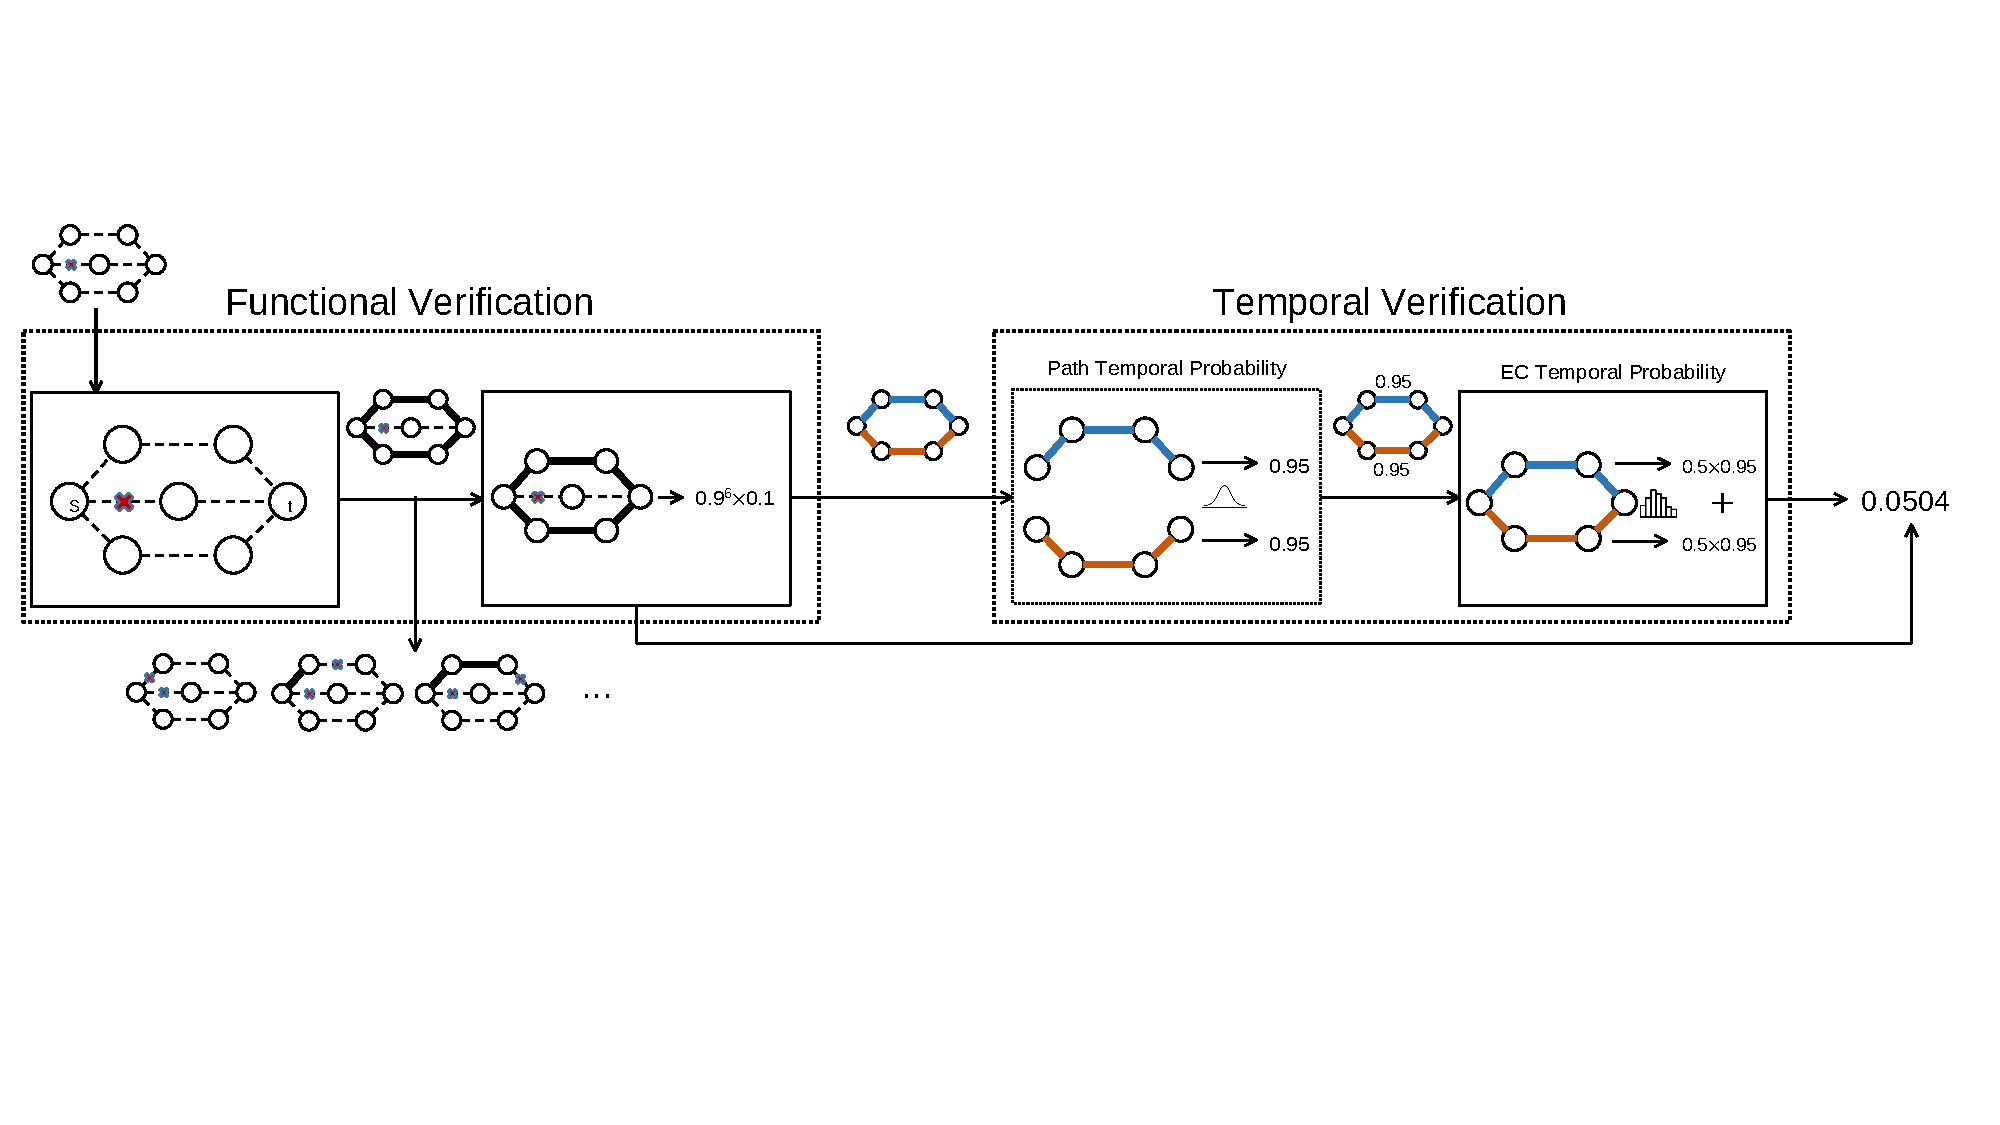
\includegraphics[scale=0.5]{overall}
    \caption{Overview of Tempus}
    \label{fig:process}
\end{figure*}

% \section{Overview}
\section{Latency Modeling Background}
In the context of verification, there are multiple approaches to model latency in a network.
We will briefly compare 4 possible methods that might be useful to attack this problem and 
and its limitation to illustrate the methodological challenge to accurately model latency.

\subsection{Simulation}
One of the available methods to reason about latency in a network is by simulating it 
using a network simulator (e.g. ns3, omnet).
On a high level, the tool will simulate the lifecycle of packets, created by a load generator, 
and the user could fail some network components and collect the packets' latency measurement 
to see how the perturbation affects the latency property in question.

Network simulator has been widely used in our community as an alternative to experimenting on 
a bare-metal system. 
While generally accurate, network simulators notoriously take a long time to run.
Moreover, the simulation workflow is more akin to testing than verification, relying on 
the user to create failure scenarios and reason about latency in a contrapositive way -- 
the absence of a negative result does not mean the property is guaranteed to be fulfilled.

\subsection{Timed Automata}
Timed Automata is an extension to the classic Finite State Machine (FSM) in automata theory that 
adds a global clock to be used as transition constraints. 
The runtime will keep a set of global clock that monotonously increases and can be individually 
reset.
Using these clocks, we could construct the state machine that constraints each transition with 
a time limit. 
With this additional time constraints, we could verify properties in a similar way 
as traditional model checking methods (e.g. using CTL formulas).

While this technique offers a proper verification framework and a higher level of abstraction 
compared to simulation, traditional Timed Automata theory is deterministic, offering no random 
transitions to express random component failure and a way to reason about latency probabilistically.

A popular Timed Automata modeling tool, UPPAAL, tried to alleviate this determinism problem by 
introducing Statistical Model Checking (SMC) on top of their Timed Automata model. 
The feature allows user to introduce random transition (with configurable weights) and distribution 
based transition, in order to probabilistically reason about the desired property and model 
random failures of network components.

However, they did it by collecting the statistical property of multiple simulation runs, which 
has the same drawback as the simulation-based method. 
It is also limited in its choice of probability distribution, only allowing user to use uniform and 
exponential distribution.

\subsection{Queuing Theory}
Another theoretical framework that is more closely related to networking devices are queuing 
theory.
Queuing theory allows you to reason about the equilibrium latency of a given traffic, given the 
arrival and processing distribution to each component, among other things.

One major downside of this framework, however, is the limitation of assumed probability 
distributions that is being used in each queue and the arrival process. 
Where one could derive a closed-form solution for a network where the queues and / or the arrival process 
are identified as a poisson process (i.e. Jackson network, BCMP network \cite{bcmp}), 
the same thing cannot be said for a queuing network that posits a more diverse queuing behavior.
A framework to describe a queuing network with an arbitrary queuing behavior and arrival process in this 
theory is yet to be discovered.

\subsection{Latency as Random Variable}
% Verification framework that is
% - Expressive (congestion control, load-balancing scheme, traffic generation -> probabilistic)
% - Performant (verification time that makes sense, proper-level of abstraction)
% - Practical (reasonably accurate while requiring minimal amount of information and assumption)

Considering these available approaches and their respective strength and limitation, we devise a 
simple yet powerful framework to verify the latency property in a given network.

Our main idea is to model the latency of a given network component as an independent random variable.
By modeling the latency this way, we could then operate on those random variable to model the latency 
of a given path, and eventually the latency of a given src-dst pair.
Using the resulting random variable, we could then determine the temporal property in question by 
analyzing the statistical property of the resulting probability distribution.

\textbf{This framework is expressive}.
The packet interarrival time that is represented by the latency distribution in each router encodes the 
latency information of the various traffic that is going through the network.
At the same time, it also encodes the effect of congestion and flow control scheme that affects 
those traffic.

\textbf{This framework is performant}.
Operating on the high-level of abstraction of the latency distribution in each network components allows 
this framework to perform the verification task in a matter of minutes?
We demonstrate our evaluation result on Section \ref{eval}.

\textbf{This framework is practical}.
Queue length is a common metric that is used to measure the resource utilization of a network 
\cite{dctcp} \cite{swift}.
Using this metric, one could easily construct a latency distribution by combining it with the 
line rate bandwidth.

% \subsection{Latency as Path Property} 
% We began our study by first pondering about a basic construct: modeling the end-to-end latency of 
% a single packet.
% In a packet-switched network, a packet is sent from one transmiting host to one receiving host 
% through the many components of the network (e.g. links, routers, firewall) and each of those 
% components might introduce some latency into the packet transmission process.
% Figuring out which of those components will actually introduce latency into the packet in question, 
% and by how much, is the next logical step that we must figure out.

% Obviously, a given packet doesn't need to visit all network components to reach its destination 
% host.
% A network engineer will configure the network in such a way that a packet will only need to be 
% routed via a specific subset of its components.
% That specific subset is dictated by two things: how those components are connected together 
% (i.e. topology) and how the control plane protocols are configured to route a packet (e.g. routing 
% protocol, ACL).
% Based on a variety of these setups, nodes in the network will form a forwarding table to route a 
% given packet appropriately.

% The goal of a classical control plane verifier then, is to use this forwarding table in some 
% form to verify certain properties. %TODO: examples?
% However, looking at the forwarding table alone will not give us a conclusive result regarding 
% which components are going to be visited by a given packet, making verification of latency 
% properties less clear.
% For example, the network might be configured with a load-balancing protocol in which a packet 
% departing from a source host might take multiple different \textit{paths} (with certain 
% probability weights) to arrive at the destination host, possibly resulting in a different 
% end-to-end latency measurement.

% Therefore, we argue that when it comes to analyzing end-to-end latency, a network path should be 
% the primary unit of reasoning, rather than forwarding table.
% By being more specific about our unit of reasoning, we could answer verification questions more 
% clearly, and we could design our verifier more efficiently since we could use it to represent 
% multiple different forwarding tables that shares the same path.

% \subsection{Relation to Classical Verifier}
% Before we analyze the latency of a given packet that propagates through a certain network 
% path however, we must make sure that said path exists in the first place.
% We note that latency is a property that only make sense after connectivity between two hosts 
% has been established. 
% In other words, if two nodes in a network aren't even functionally connected (e.g. physical 
% link failure, ACL policy), then the latency between them will \textit{always} be infinite, 
% making the verification task trivial.

% Fortunately, there are a rich body of work in the network verification literature regarding 
% functional reachability under failure. %TODO: cite
% We could then design our verifier on top of an existing classical control plane verifier.
% We use it to verify reachability property, and only if the reachability property is fulfilled, 
% we would verify whether the latency between two hosts fulfilled some additional condition.

% \subsection{Path Latency Distribution}
% Up to this point, we have talked about measuring the latency of a single packet by figuring out 
% its path; analyzing which exact components it has traversed through.
% However, when we try to generalize this framework and ask questions about the latency of multiple 
% packets, it is apparent that the path alone is not a determinative information, as the latency 
% of two packets propagating through the same path might be different due to a multitude of factors.

% The natural extension to the framework then, is instead of representing latency of a path with a 
% single number, we instead represent it with a continuous random variable that signifies the 
% possible delay that a given packet traversing through that path might have.
% This random variable will have a distribution that marginalizes over all other factors other than 
% the path.

% We can then use this latency distribution to verify some temporal properties in a probabilistic 
% manner.
% For example, we could verify the probability that a packet will be delivered in under a time 
% unit by taking the CDF of the distribution.

% \subsection{Path Decomposition and Convolution} \label{decomposition}
% The final question that we had to decide on was how do we actually model path latency distribution
% based on real component measurements.
% Considering the complexity of factors that might determine the path latency distribution and the 
% availability of measurement data, we settle on the assumption that the path latency distribution 
% is composed of multiple independent distribution that corresponds to the latency each components 
% in the path might introduce.
% %TODO: confirm about independence?

% Since not all components in the path will introduce latency with a non-negligible value, we 
% specifically choose to model two source of latency in the path's components which we deem 
% significant: \textbf{link propagation latency} and \textbf{queuing latency}.
% %TODO: expand on how to get the data later

% Propagation delay is the latency that is introduced by the links in the network, which is 
% independent of the traffic load in the system.
% Queuing delay is the latency that the queuing process in the node introduced. 
% Unlike propagation delay, queuing delay might be dependent on load in the system, since the more 
% packets there are in the queue, the more delay the node will introduce to a subsequent packets.

% For propagation delay, the semantic of this random variable is relatively straightforward: it is 
% the distribution of latency that a given link will introduce.
% For queuing delay however, this random variable represents the delay that a given queuing process 
% will introduce, marginalized over various traffic pattern that a given network state might have 
% resulted.

% In order to obtain the overall path latency distribution from these per-component latency 
% distributions, we do a convolution operations over all the relevant component's latency 
% distributions.
% Since not all distributions can be convolved in a closed-form fashion, we use a numerical 
% convolution technique with a guaranteed error bound. 
% We initially consider a Monte-Carlo simulation in order to approach numerical convolution, but 
% the lack of a general technique to measure error made us opt for the formerly mentioned method.


% \section{Verifier Design}

We divide the problem of latency verification in this framework into two parts: 
verifying that two nodes are reachable (\textbf{functional verification}) and only if 
the functional property is fulfilled, we would verify whether the latency between 
two nodes fulfilled some temporal condition (\textbf{temporal verification}).
In Section \ref{sec:functional}, we briefly describe the functional verification scheme that 
our framework is built upon. 
Next, in Section \ref{sec:temp}, we describe our novel temporal verification framework 
in more detail.
Next, in Section \ref{sec:opt}, we describe the optimization techniques that arise from 
these two steps.
We then evaluate our implementation in Section \ref{eval}.
Finally, we will touch on some related works on Section \ref{sec:rel}, limitations and future 
works on \ref{sec:fut}, and conclude our work with Section \ref{sec:conc}.

\section{Functional Verification}
For functional property verification, NetDice \cite{netdice} 
has laid the way for verifying reachability between two nodes under failure in a 
probabilistic and efficient manner.
To contextualize our modification, we will briefly describe some parts of 
NetDice's network encoding and exploration algorithm as a prelude to our alteration.
For a more complete complete description of NetDice, please refer to the original 
paper.

\begin{figure}[h]
    \centering
    % \includegraphics[width=0.4\textwidth, trim=0cm 11cm 0cm 5cm]{ex.pdf}
    \includegraphics{../tikz/ex}
    % \includegraphics{ex.eps}
    \caption{Example topology, we want to check the reachability of A to Z}
    \label{fig:ex}
\end{figure}

\subsection{Topology Graph}
In this framework, a network is encoded in an edge-labeled directed graph 
$G_t = (V_t, E_t)$ where $V_t$ represents the nodes in the network and 
$E_t$ represents the functional connectivity between a source and a destination node. 
A physical link is then represented as a pair of symmetrical edges that shares the same source 
and destination node but with opposite direction (e.g. $v_1 \rightarrow v_2$ and $v_2 
\rightarrow v_1$).
A routing protocol is then defined on top of this graph by some auxilary information.

To explain it with further clarity, we use the topology in Fig. \ref{fig:ex} as a 
running example for this paper. 
We will assume that the nodes in the network runs OSPF with weight 1 for every edge and ECMP 
as their load-balancing scheme.
We want to check the temporal probability of packets that departs from A to Z.

% To represent the component's random failure, NetDice defined two failure rates.
% The first failure rate is the chance that a given physical link in the network will go down.
% The second failure rate is the chance that a given node in the network will go down.
% These rates are shared between all links / nodes in the network.
% Internally however, the node failure rate will be translated into the link failure rate 
% with a Bayesian Network model, since a node failure can be modeled with the failure of each 
% links connected to it.

To represent random failure, NetDice defined a universal link failure rate (i.e. 
the probability of \textit{any} link in the network randomly failing).
We refine NetDice's model slightly by allowing each links to have different failure rate.
We label each edge in $E_t$ with a function $r: E_t \rightarrow \{x \in \mathbb{R} \mid 0 \le x 
\le 1\}$ that represents the failure rate of a given physical link.
As a consequence, two symmetrical edges (i.e. two edges that shares the same node pairs but with 
opposite direction) will also share the same failure rate, and will be disabled in a coupled 
fashion.

For the sake of example, in our Fig. \ref{fig:ex} topology, we will assume that each link has a 
10\% chance of failure.

% \subsubsection{Routing}
% On top of this topology, NetDice also defined additional informations that would be used
% by a routing protocol to determine the valid path(s) between two nodes $src, dst \in V_t$ given 
% a particular link failure scenario. 
% These routing informations would also be used by their optimization algorithms to reduce the 
% amount of states that are going to be explored.

% NetDice implemented iBGP and OSPF (with ECMP) routing protocols.
% They encode the relevant routing information by assigning some labels to the vertices or edges
% in the topology.
% In OSPF for example, we define a function $w_{ospf}: E_t \rightarrow \mathbb{N}$ as the edge-label 
% that represents the positive weight of a link.
% They would later be used to compute the convergent paths of a given network state 
% (\ref{verification}).

\subsection{State Exploration}
A \textbf{network state} is defined as a set of failed links.
There are $2^{|E_t|}$ network states in a given network and a brute-force strategy 
would need to explore all of the states to compute the reachability property of a 
node pair in a given network. 
NetDice however, will merge multiple network states into an \textbf{equivalence class}
by marginalizing over \textit{cold edges}, links whose failure is guaranteed not to 
change the convergent path of a highlighted network state.

NetDice will systematically explore many equivalence classes in the network. 
It will start from the equivalence class of a perfect network and will fail certain 
\textit{hot edges} (i.e. edges that are not cold) to explore another equivalence 
class.
While not explicit in its description, NetDice's algorithm will effectively form an 
\textbf{exploration tree}. 

In order to preserve some information that will be used in the temporal verification 
stage, we modify this original exploration algorithm to make it more explicit.
We started by formalizing the notion of Equivalence Classes.
An Equivalence Class $\mathcal{E}$ is defined as a 3-tuple $(U_h, D_h, paths)$.
$U_h$ and $D_h$ refers to a set of hot edges that are up and down respectively.
$paths$ refers to the convergent paths between src-dst pair that is produced by the
control plane when the links in $D_h$ fails.
Unlike the original algorithm, we explicitly store $paths$ in $\mathcal{E}$ so that 
it could be used to for the temporal verification stage.

We then define the Exploration Tree $\mathcal{T}$ as a tree of Equivalence Classes.
At the root, we have an Equivalence Class that corresponds to a perfect network, where 
$paths$ is the path(s) that the control plane will produce given a perfect network 
condition and $U_h = D_h = \emptyset$.
Each Equivalence Class in this tree will have children which have one of its parent's link in 
$paths$ appended to its $D_h$, essentially failing one of the link in the path.
If an Equivalence Class has an empty $paths$, then it would have no children.

To compute the functional probability $P_f$ of a given Equivalence Class, we compute the 
product of the 'up' probability of all the links in $U_h$ and $paths$ and the 
product of the 'down' probability of all the links in $D_h$.

In our running example, we could see the subset of the exploration tree in Fig. 
\ref{fig:tree}. 
We see that in a perfect network ($\mathcal{E}_1$), OSPF will produce $ACZ$ as the 
shortest path between A to Z.  
The probability of this Equivalence Class actually materializing ($P_f$) is $0.81$, 
which is the probability of $AC$ and $CZ$ being up at the same time ($0.9^2$).

In the Equivalence Class where the link $AC$ is failing however ($\mathcal{E}_2$), 
OSPF and ECMP will produce two equaly-weighted paths $ABEZ$ and $ADFZ$.
The probability of this Equivalence Class actually materializing ($P_f$) is $0.053$
($0.9^6 \cdot 0.1$).

After having the algorithm produced $\mathcal{T}$, we then continue to the temporal verification 
stage.

\section{Temporal Verification} \label{sec:temp}
In the temporal verification stage, we will use the path information that we got from 
functional verification stage and augment them with latency information to 
produce the final temporal property probability.

\begin{figure}[h]
    \centering
    % \includegraphics[width=0.4\textwidth, trim=0cm 11cm 0cm 5cm]{ex.pdf}
    \includegraphics[width=\columnwidth]{../tikz/tree}
    % \includegraphics{ex.eps}
    \caption{Subset of Modified Exploration Tree $\mathcal{T}$ for our example topology, 
        $\mathcal{E}_2$ and $\mathcal{E}_3$ will get consolidated}
    \label{fig:tree}
\end{figure}

\subsection{Latency Label}
Similar to link failure $r$, we use edge-labeling technique to represent latency that 
will get introduced by the connectivity between two nodes. 
Our model will model two significant sources of latency: \textbf{link propagation} 
and \textbf{packet queuing in the node}.
We will encode these latencies by equipping the model with two additional labels.

Encoding link propagation latency is fairly straightforward. 
We define a function $l_p: E_t \rightarrow \mathcal{D}$ where $\mathcal{D}$ is a set of 
continuous univariate distribution that has a minimum value of $0$.
This distribution signifies the time it would take for the respective physical link to transmit 
a packet from one end to another.
Because of this, just like $r$, two symmetrical edges will share the same distribution.

To encode queuing latency, we first note that the queuing mechanism in modern switches 
usually resides in the output port. %TODO: Cite PISA?
Since a port in a switch is only connected to one other port, we could effectively 
assign the latency to the connectivity between switches.
To do this, we define another function $l_q: E_t \rightarrow \mathcal{D}$.
This distribution signifies the output queue latency in the source node that is 
going to be forwarded to the destination node.
Unlike $l_p$, two symmetrical edges will have two different distributions since they 
represent two different output queues.

In our running example, we will assume that all edges in the topology will have $l_p$
and $l_q$ of gamma distribution with $\lambda = 1$, except $l_q(EZ)$ which will 
have a lognormal distribution with $\alpha = 1$ and $\theta = 1$.

Given $paths$, $l_p$, and $l_q$, we could then compute $P_t$, the probability of a 
given temporal property being fulfilled.
We will describe our algorithm for computing this probability in the next few 
sections.

\subsection{Weighted Average and Path Convolution}
Since a convergent behavior of the forwarding plane $paths$ might contain more than 
one paths, we will compute the temporal probability of $paths$ by computing the 
weighted average of the temporal probability of each of the individual path.
The specific weight depends on the load-balancing method used.
%We have implemented the weight computation for ECMP load-balancing scheme.

To get the temporal probability of a single path, we will use the latency information 
from $l_p$ and $l_q$ to compute the latency distribution of the whole path.
To do this, we resort to the methods of \textbf{convolution}.
For each edge $e$ in the path, we will get $l_p(e)$ and $l_q(e)$ and convolve them 
all together to get the path latency distribution.

With this path latency distribution, we could get the temporal probability of a 
path by computing the statistical property of said distribution.
In this work, given a path latency distribution $\mathcal{L}$, we define two temporal 
properties:
\begin{itemize}
    \item \textbf{Bounded Reachability}: the probability that a packet will get 
        transmited below $t$ time unit. This will get computed as $cdf(\mathcal{L}, t)$
    \item \textbf{Tail Reachability}: the probability that a packet will get 
        transmited above $t$ time unit. This will get computed as 
        $1 - cdf(\mathcal{L}, t)$
\end{itemize}

In our Fig. \ref{fig:tree} Exploration Tree for example, $\mathcal{E}_2$ has two 
equally probable path, $ABEZ$ and $ADFZ$.
We will first do a chain convolution of all the distributions in $ABEZ$ ($l_p(AB)$, 
$l_q(AB)$, ..., $l_q(EZ)$) and do the same thing for $ADFZ$.
We will then take the $CDF$ of $\mathcal{L}_{ABEZ}$ and $\mathcal{L}_{ADFZ}$ with our 
desired $t$ and average them out to get $P_t$ of $\mathcal{E}_2$. 

In short, given $paths$, $l_p$, and $l_q$, we will do the following:
\begin{enumerate}
    \item Split $paths$ into its individual path
    \item For each path, compute its latency distribution by convolving the latency distribution 
        $l_p$ and $l_q$ of each link
    \item With the resulting path latency distribution, determine the probability of temporal 
        property by computing the statistical property of said distribution
    \item Combine the temporal property of each path by computing the weighted average, based 
        on the load-balancing scheme of the control plane
\end{enumerate}

We do each of these steps to every Equivalence Class in $\mathcal{T}$, and do a sum-product operation 
of $P_f$ and $P_t$ to get the final probability of the property in question.

By introducing the temporal verification algorithm, we're essentially adding additional overhead to the 
exploration algorithm (on top of functional verification) that scales to the size of the Exploration Tree.
In other words, for $\mathcal{T}$ of size $n$, we will need to do temporal verification in each of 
those $n$ Equivalence Class.
We aim to minimize the overhead of temporal verification by introducing some optimization algorithms
later.

\subsection{Numeric Convolution}
However, there is one major problem with a convolution-based technique for computing the latency distribution 
of a given path: not every distribution pair can be convolved analytically.
A closed-form solution of a convolution is usually only available for two distributions of the same type.

In our example, we define $l_q(EZ)$ to be lognormal distribution, which doesn't have a closed form convolution 
solution with the other latency distribution in the network, which is of gamma distribution form.
Therefore, in order to convolve two arbitrary distributions, we need to leverage a numerical convolution 
method.

We leverage an existing numerical convolution algorithm, DIRECT, to fulfill this role.
%TODO: describe DIRECT in one sentence
We choose this method due to their bounded error property: DIRECT guarantee that the computed 
distribution and the correct theoretical distribution has a KL-divergence below a certain bound.
DIRECT has also been implemented in R's popular bayesmeta package.
%TODO: cite and change font?

One subtle detail about DIRECT is while convolution is defined to be a commutative operation, and 
DIRECT also achieves this property, the order of operation matters for the algorithm's runtime 
performance.
In particular, if we had a chain of DIRECT convolutions, the result of a convolution should not be set 
as the second input distribution in the later convolutions to avoid performance penalty.
This is caused by a nested loop from the following two mechanisms:
\begin{itemize}
    \item DIRECT works by computing a list of support values by doing many PDF queries of the second input
        distribution
    \item Computing the PDF of a DIRECT distribution (the returned distribution of a DIRECT 
        algorithm) itself involves iterating over the current support values
\end{itemize}

As an ilustration, if we had 3 random variables $A$, $B$, and  $C$, and we want 
to convolve them all together, it would be faster to compute $direct(direct(A, B), C)$ instead of 
$direct(C, direct(A, B))$.

While this problem is trivial to solve (swap the input parameter if the latter is detected as a 
DIRECT distribution), it does limit the type of optimization that we could have in the chain convolution 
process.

\section{Optimization} \label{sec:opt}
\subsection{Equivalence Class Consolidation}
To minimize the amount of temporal verification overhead, we want to find some symmetry in the 
existing exploration algorithm so that we could reduce the exploration space even further.

In the original NetDice exploration algorithm, multiple network states were merged into an Equivalence 
Class based on its cold edges (edges whose failure won't change the convergent path(s)).
In other words, network states within the same Equivalence Class will have the same convergent path(s).

However, we observe that each of those Equivalence Classes are not \textit{unique}: while network states within 
the same equivalence class shares a convergent path(s), \textbf{multiple equivalence classes could also 
share the exact same convergent path(s)}, as shown in $\mathcal{E}_2$ and $\mathcal{E}_3$ in Fig. \ref{fig:tree}.

Since we define latency distribution to marginalize over all factors other than the path, we could 
effectively \textit{consolidate} these equivalence classes into one big equivalence class and do temporal 
verification once.

We implemented this idea by doing memoization on the temporal probability of a given convergent path(s).
We will only do temporal probability computation once, when we first iterate over an equivalence class that 
has a certain convergent path(s), and we cached the result should another equivalence class with the same 
convergent path(s) emerged.

\subsection{Path Memoization}
After consolidating many equivalence classes that shares the same convergent path(s), we are left with fewer, 
bigger, but unique equivalence classes.
As significant as it is, we could reduce the computation cost further by drawing connections between these 
unique equivalence classes.

In a network with a load-balancing protocol, the convergent state of the data plane might forward a packet 
through multiple possible paths.
In the context of our framework, we say that an equivalence class might have more than one convergent paths.
Nevertheless, we note that two equivalence classes with different convergent paths might not be two 
independent subset.
In other words, \textbf{multiple equivalence classes could share a subset of individual path}.

Since the way we compute convergent path(s) temporal probability is by calculating the weighted average of 
individual path temporal probability, we could reduce the amount of convolution we will need to do by doing further memoization 
on the temporal probability of a given path.
If we were to compute the temporal probability of an equivalence class with previously cached individual 
path, we only need to calculate the weights that corresponds to the load balancing protocol without 
doing any convolution.

In our running example, we could see that in Fig. \ref{fig:tree}, $\mathcal{E}_2$ and $\mathcal{E}_4$ share 
an identical path, $ADFZ$.
We could therefore memoize $cdf(\mathcal{L}_{ADFZ}, t)$ when we explore $\mathcal{E}_2$ and query the 
cached result when we explore $\mathcal{E}_4$.

With this optimization, we will do a chain convolution by the amount of path available in the network between 
the source and destination (which is 3 in the case of our running example in Fig. \ref{fig:ex}: $ACZ$, $ABEF$, 
and $ADFZ$).

\subsection{Convolution Grouping}
Aside from optimizing the \textit{amount} of paths we need to do convolution on, we could also do some 
optimization on the \textit{convolution operation itself}. 

\begin{figure}[h]
    \centering
    % \includegraphics[width=0.4\textwidth, trim=0cm 11cm 0cm 5cm]{ex.pdf}
    \includegraphics[width=\columnwidth]{../tikz/group}
    % \includegraphics{ex.eps}
    \caption{One example of a convolution tree to get $\mathcal{L}_{ABEZ}$ with optimized grouping,
    we want to start introducing numerical convolution as late as possible}
    \label{fig:grouping}
\end{figure}

While the use of numerical technique to do convolution enabled us to use arbitrary probability distribution 
in our framework, it comes with two noticeable disadvantages.

The first is \textit{error}: numerical method is fundamentally an approximation technique that always 
comes with some error. 
While DIRECT algorithm comes with an error-bound guarantee, it is not zero and could expand if we do 
chain convolution.

The second is \textit{runtime performance}: even with the input ordering constraints we laid out on the 
previous subsection, DIRECT is still generally slower than analytical convolution.
This is expected, since a closed form solution of a convolution tipically boils the operation down into 
a few arithmetic calculation, rather than complex operation like integration.
Due to these factors, we feel the need to \textbf{prioritize analytical convolution} in the calculation of 
path latency distribution.

We did this by \textit{grouping} subsets of the path components with the same probability distribution 
type (e.g. exponential, normal, etc.). 
We then analytically convolve the distribution within that subset and only numerically convolve the 
returned distribution, which will be fewer in quantity, thus enabling smaller error and faster performance.

In our running example, in the chain convolution process to get $\mathcal{L}_{ABEZ}$, we will analytically
convolve $l_p(AB)$, $l_q(AB)$, $l_p(BE)$, $l_q(BE)$, and $l_p(EZ)$ since they are of the same type (gamma) 
and then numerically convolve the resulting distribution with $l_q(EZ)$.
Fig. \ref{fig:grouping} illustrates how the chain convolution process will be broken down.

% \textbf{First}, we do the functional verification with $G_t$ similar to what NetDice 
% \cite{netdice} have done. 
% In addition, we also collect additional information from each state (e.g. convergent 
% paths) to be used in the temporal verification step. 

% \textbf{Second}, we compute the total path latency distribution from the convergent path(s) in each 
% state with $G_l$.
% This is done by convolving over the latency distribution of each component in the path. 
% Since not all convolutions can be calculated analytically, we implemented a numerical convolution 
% method via mixture distribution, DIRECT \cite{rover2017discrete}, which is able to convolve two 
% distribution with a KL divergence error bound.
% Multiple states can share the same convergent path(s), so \textit{only a fraction of the states need to be 
% explored}.

% \textbf{Third}, we calculate the probability of a given temporal property being true in that state. 
% For example, given a \textit{bounded reachability property} (probability of whether a packet can 
% traverse from a source to destination below some time unit $T$), we can compute its probability by 
% integrating the PDF from $0$ to $T$. 
% We then combine all of the \textit{temporal} and \textit{functional} probability in each state to 
% get the final probability: the probability of \textit{the network} fulfilling a temporal property.

% TODO: intro, reformalize graph formulation, citations
% Does a figure about topology graph and latency graph will be useful?
% Multimedia context on older networked system Klara Nahrstedts
% Graph 

\section{Optimization} \label{sec:opt}
\subsection{Equivalence Class Consolidation}
To minimize the amount of temporal verification overhead, we want to find some symmetry in the 
existing exploration algorithm so that we could reduce the exploration space even further.

In the original NetDice exploration algorithm, multiple network states were merged into an Equivalence 
Class based on its cold edges (edges whose failure won't change the convergent path(s)).
In other words, network states within the same Equivalence Class will have the same convergent path(s).

However, we observe that each of those Equivalence Classes are not \textit{unique}: while network states within 
the same equivalence class shares a convergent path(s), \textbf{multiple equivalence classes could also 
share the exact same convergent path(s)}, as shown in $\mathcal{E}_2$ and $\mathcal{E}_3$ in Fig. \ref{fig:tree}.

Since we define latency distribution to marginalize over all factors other than the path, we could 
effectively \textit{consolidate} these equivalence classes into one big equivalence class and do temporal 
verification once.

We implemented this idea by doing memoization on the temporal probability of a given convergent path(s).
We will only do temporal probability computation once, when we first iterate over an equivalence class that 
has a certain convergent path(s), and we cached the result should another equivalence class with the same 
convergent path(s) emerged.

\subsection{Path Memoization}
After consolidating many equivalence classes that shares the same convergent path(s), we are left with fewer, 
bigger, but unique equivalence classes.
As significant as it is, we could reduce the computation cost further by drawing connections between these 
unique equivalence classes.

In a network with a load-balancing protocol, the convergent state of the data plane might forward a packet 
through multiple possible paths.
In the context of our framework, we say that an equivalence class might have more than one convergent paths.
Nevertheless, we note that two equivalence classes with different convergent paths might not be two 
independent subset.
In other words, \textbf{multiple equivalence classes could share a subset of individual path}.

Since the way we compute convergent path(s) temporal probability is by calculating the weighted average of 
individual path temporal probability, we could reduce the amount of convolution we will need to do by doing further memoization 
on the temporal probability of a given path.
If we were to compute the temporal probability of an equivalence class with previously cached individual 
path, we only need to calculate the weights that corresponds to the load balancing protocol without 
doing any convolution.

In our running example, we could see that in Fig. \ref{fig:tree}, $\mathcal{E}_2$ and $\mathcal{E}_4$ share 
an identical path, $SDET$.
We could therefore memoize $cdf(\mathcal{L}_{SDET}, t)$ when we explore $\mathcal{E}_2$ and query the 
cached result when we explore $\mathcal{E}_4$.

With this optimization, we will do a chain convolution by the amount of path available in the network between 
the source and destination (which is 3 in the case of our running example in Fig. \ref{fig:ex}: $SAT$, $SBCT$, 
and $SDET$).

% \subsection{Convolution Grouping}
% Aside from optimizing the \textit{amount} of paths we need to do convolution on, we could also do some 
% optimization on the \textit{convolution operation itself}. 

% \begin{figure}[h]
%     \centering
%     % \includegraphics[width=0.4\textwidth, trim=0cm 11cm 0cm 5cm]{ex.pdf}
%     \includegraphics[width=\columnwidth]{../tikz/group}
%     % \includegraphics{ex.eps}
%     \caption{One example of a convolution tree to get $\mathcal{L}_{ABEZ}$ with optimized grouping,
%     we want to start introducing numerical convolution as late as possible}
%     \label{fig:grouping}
% \end{figure}

% While the use of numerical technique to do convolution enabled us to use arbitrary probability distribution 
% in our framework, it comes with two noticeable disadvantages.

% The first is \textit{error}: numerical method is fundamentally an approximation technique that always 
% comes with some error. 
% While DIRECT algorithm comes with an error-bound guarantee, it is not zero and could expand if we do 
% chain convolution.

% The second is \textit{runtime performance}: even with the input ordering constraints we laid out on the 
% previous subsection, DIRECT is still generally slower than analytical convolution.
% This is expected, since a closed form solution of a convolution tipically boils the operation down into 
% a few arithmetic calculation, rather than complex operation like integration.
% Due to these factors, we feel the need to \textbf{prioritize analytical convolution} in the calculation of 
% path latency distribution.

% We did this by \textit{grouping} subsets of the path components with the same probability distribution 
% type (e.g. exponential, normal, etc.). 
% We then analytically convolve the distribution within that subset and only numerically convolve the 
% returned distribution, which will be fewer in quantity, thus enabling smaller error and faster performance.

% In our running example, in the chain convolution process to get $\mathcal{L}_{ABEZ}$, we will analytically
% convolve $l_p(AB)$, $l_q(AB)$, $l_p(BE)$, $l_q(BE)$, and $l_p(EZ)$ since they are of the same type (gamma) 
% and then numerically convolve the resulting distribution with $l_q(EZ)$.
% Fig. \ref{fig:grouping} illustrates how the chain convolution process will be broken down.

% \textbf{First}, we do the functional verification with $G_t$ similar to what NetDice 
% \cite{netdice} have done. 
% In addition, we also collect additional information from each state (e.g. convergent 
% paths) to be used in the temporal verification step. 

% \textbf{Second}, we compute the total path latency distribution from the convergent path(s) in each 
% state with $G_l$.
% This is done by convolving over the latency distribution of each component in the path. 
% Since not all convolutions can be calculated analytically, we implemented a numerical convolution 
% method via mixture distribution, DIRECT \cite{direct}, which is able to convolve two 
% distribution with a KL divergence error bound.
% Multiple states can share the same convergent path(s), so \textit{only a fraction of the states need to be 
% explored}.

% \textbf{Third}, we calculate the probability of a given temporal property being true in that state. 
% For example, given a \textit{bounded reachability property} (probability of whether a packet can 
% traverse from a source to destination below some time unit $T$), we can compute its probability by 
% integrating the PDF from $0$ to $T$. 
% We then combine all of the \textit{temporal} and \textit{functional} probability in each state to 
% get the final probability: the probability of \textit{the network} fulfilling a temporal property.

% TODO: intro, reformalize graph formulation, citations
% Does a figure about topology graph and latency graph will be useful?
% Multimedia context on older networked system Klara Nahrstedts
% Graph 

\section{Evaluation} \label{eval}

We implemented Tempus in $\sim600$ lines of Julia \cite{julia} code.
This code will take a topology configuration, source and destination node, and the 
temporal property in question and its threshold.
It will then output the final probability of the network upholding that temporal property.
We ran our prototype on a machine with 2 Intel E5-2630 v3 8-core CPU running up to 2.4 GHz 
and 128 GB of ECC RAM, provided by CloudLab \cite{cloudlab}.

To appraise the viability of our approach, we seek to answer 5 evaluation questions:
\begin{enumerate}
    \item How long does it take to run the verifier overall? How does it scale?
    \item What is the bottleneck step in the verification process?
    \item How effective is the optimization technique in reducing the verification time?
    \item How effective is the optimization technique in reducing the explored equivalence classes?
    \item How does different topologies affect optimization effectiveness?
\end{enumerate}

\subsection{Experiment Setup}

\begin{table}[h]
    \begin{tabular}{| c | c | c | c |}
    \hline
    Topology & \#routers & \#links & type \\
    \hline
    Fat Tree 4 & 20 & 32 & DC \\
    Fat Tree 6 & 45 & 108 & DC \\
    Fat Tree 8 & 80 & 256 & DC \\
    Fat Tree 10 & 125 & 500 & DC \\
    Fat Tree 12 & 180 & 864 & DC \\
    Fat Tree 14 & 245 & 1372 & DC \\
    Fat Tree 16 & 320 & 2048 & DC \\
    Fat Tree 24 & 720 & 6912 & DC \\
    Fat Tree 32 & 1280 & 16384 & DC \\
    Latnet & 69 & 74 & WAN \\
    Highwinds & 18 & 31 & WAN \\
    AT\&T & 25 & 56 & WAN \\
    Uninett & 74 & 101 & WAN \\
    GtsCe & 149 & 193 & WAN \\
    \hline
\end{tabular}
\caption{List of topologies being tested}
\label{tab:topologies}
\end{table}

We tested Tempus on 5 real-world WAN topologies from the Topology Zoo and 3 datacenter topologies 
(fat-tree, with various amount of pods).
%TODO: stats of the topologies

\subsubsection{Functional Verification}
As verifying the routing protocol functional behavior is not the primary contribution of our research, 
we simply use OSPF as the routing protocol in our experiment with uniform link weights of 1.
We set 0.1\% failure rate in all links, in accordance to the failure rate in previous studies. %TODO: cite
We then run the functional verification with $10^{-8}$ inaccuracy level.

In order for our evaluation to be realistic, we set the source and destination node to be one of the 
edge routers (node with the smallest degree / smallest centrality?).
%TODO: edge-to-edge routers

\subsubsection{Temporal Verification}
For latency distribution, we show that we can use an empirical measurement as a distribution by 
using the reported queue length from DCTCP \cite{dctcp}.
By multiplying the queue length distribution with the line-rate, we could approximate the queuing 
latency distribution for a given router. 

Since the CDF operation that we define for temporal property verification is relatively cheap, 
we expect our result to generalize with any threshold we chose. 
In other words, while changing the threshold will change the final probability, it won't change 
the runtime performance of Tempus.
Thus, we set an arbitrary threshold for our evaluation.

\subsection{Runtime Profiling}

\begin{figure}[h]
    \centering
    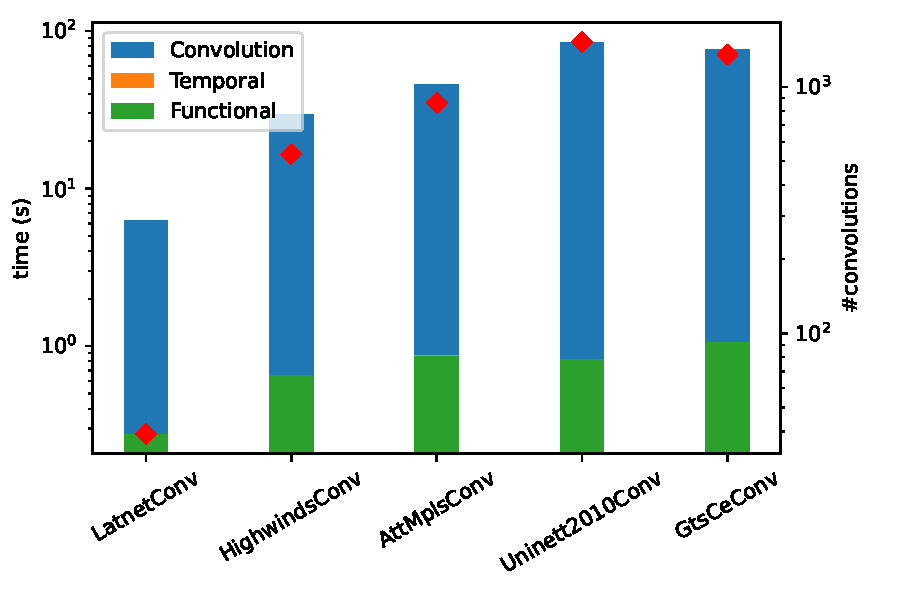
\includegraphics[scale=0.5]{scalability}
    \caption{Runtime performance of the verification process, red dots represent the number of convolutions}
    \label{fig:scalability}
\end{figure}

\begin{figure}[h]
    \centering
    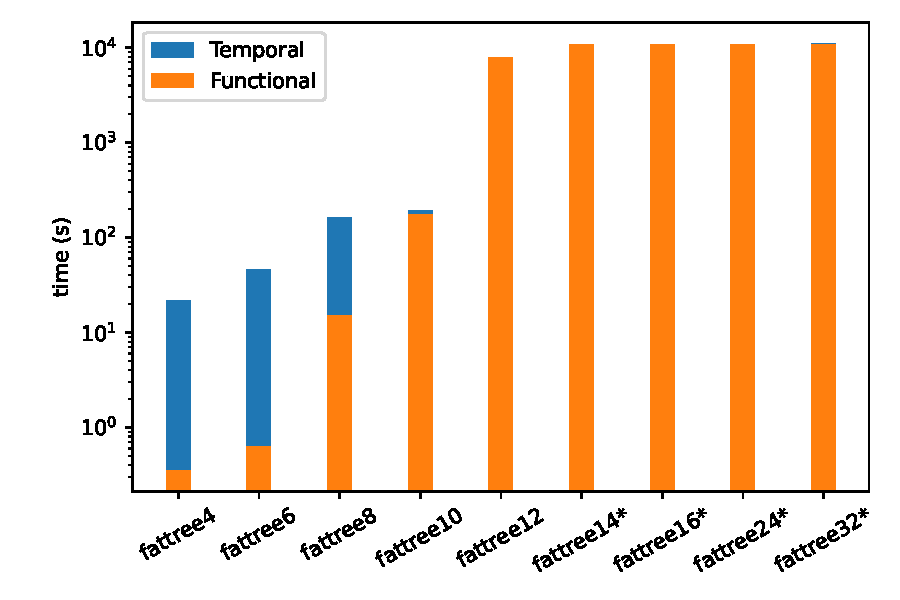
\includegraphics[scale=0.5]{scalability_fattree}
    \caption{Fat Tree, red dots represent the number of convolutions}
    \label{fig:scalabilityfat}
\end{figure}

\subsubsection{Performance and Scalability}
To begin our evaluation, we first measured the running duration of the verification process (and its steps) 
on various topologies.
Our results in Fig. \ref{fig:scalability} shows that our verification technique finished within a reasonable timeframe.
The verifier finished in the order of minutes, even for topologies with hundred of nodes.

From the same result, we also note that our verifier scales gracefully over the size of the network.
The verification duration ranges from 6 seconds to around 15 minutes. 
% TODO: fat-tree scalability
To drive this point more precisely, we also evaluate the running time of fat-tree topology in various sizes.
Our results in Fig. \ref{fig:scalabilityfat} shows that by keeping the same type of topology and scaling them up, we increased 
our verification time almost linearly, while the unoptimized version timed out after 2 hours.
Not only that, our combined optimization strategies actually reduces the time for fat tree topology of $k=10$ compared to 
equivalent topologies with smaller size.

\subsubsection{Bottleneck}
By looking at the proportion of time spent on each step in Fig. \ref{fig:scalability}, we could see that 
the combined \textbf{convolution procedure is the bottleneck} step in our verifier.
The convolution procedure takes 95\% - 99\% of the duration of the overall verification.
Hence we can see in the same figure that the runtime performance of Tempus and the total amount 
of convolution is highly correlated.

We conclude that for a reasonably low imprecision level, \textbf{Tempus runs in the order of 
minutes} and the performance of Tempus is primarily \textbf{bottlenecked by the total convolution 
operations}.

\subsection{Optimization Effectiveness}

\begin{figure}[h]
    \centering
    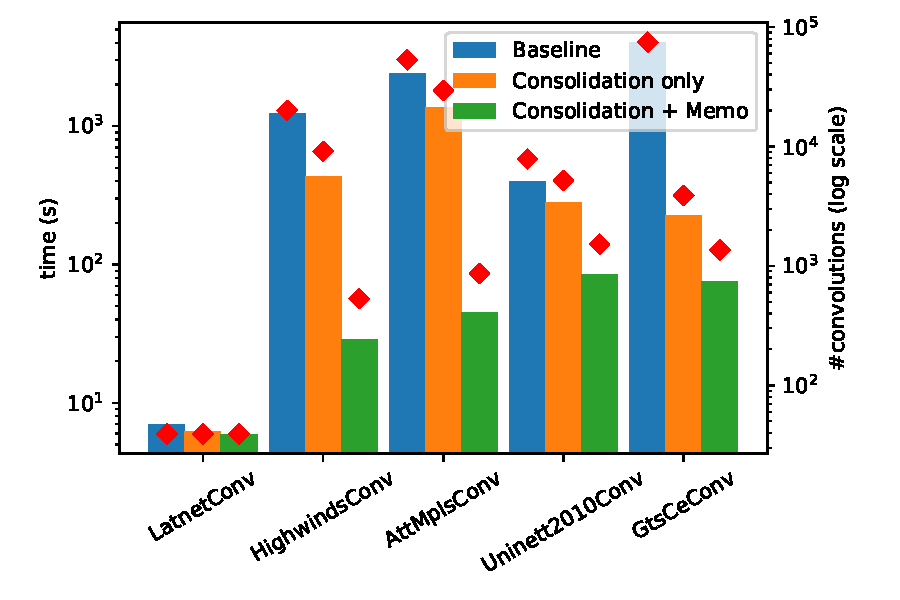
\includegraphics[scale=0.5]{optimization}
    \caption{Amount of convolution (in log scale) depending on what optimization strategy is applied}
    \label{fig:opt}
\end{figure}
\begin{figure}[h]
    \centering
    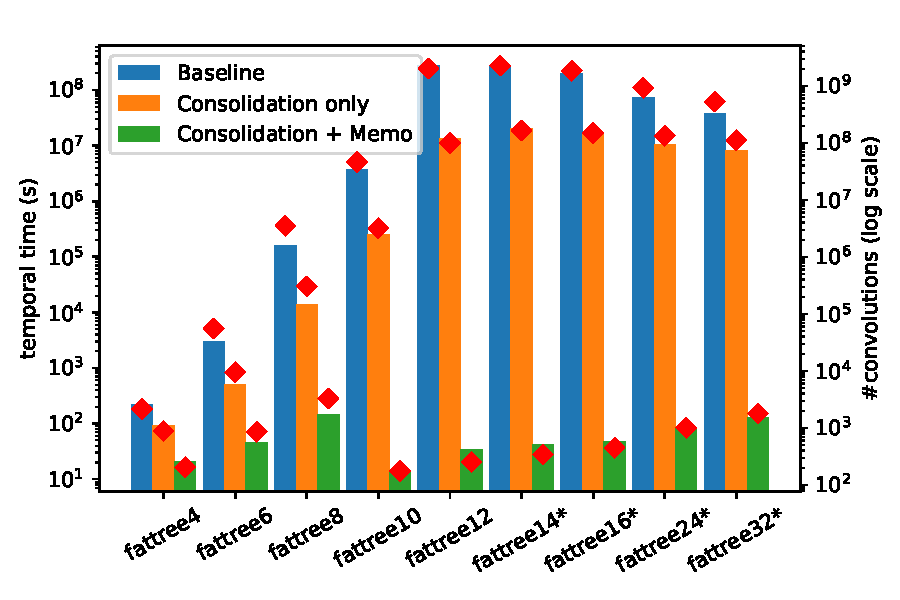
\includegraphics[scale=0.5]{optimization_fattree}
    \caption{Amount of convolution (in log scale) depending on what optimization strategy is applied. 
        Fattree 12 upwards is extrapolatied from the number of convolution}
    \label{fig:opt_fat}
\end{figure}

We have established that the convolution procedure is a relatively expensive operation within 
our verifier.
Next, we inspected the effectiveness of our optimization techniques in reducing them.
To do that, we measured the overall running duration of the verifier while selectively disabling the 
optimization.

Our results in Fig. \ref{fig:opt} shows the effect of the two optimization techniques we introduced -- 
consolidation and memoization -- in reducing the verification duration and amount of convolution (both in log scale).
For baseline, we ran the verifier without any optimization, resulting in the left bar.
The middle bar represents the result where we enable only the consolidation strategy.
Finally, the right bar represents the result where we enable both the consolidation and memoization strategy.

We note that for most of the topologies, the combination of both optimization strategies resulted in 
\textbf{79\% - 98\% improvement in performance}.
Compared to the baseline performance, the consolidation strategy contributes to 30\% - 94\% of the improvement and
the memoization strategy contributes to 67\% - 96\% on top of that. 
%TODO: factors of the network node-pair? path amount and length?

We conclude that \textbf{consolidation and memoization are both effective optimization strategies} in our verification
framework.

\subsection{Equivalence Class Reduction}

\begin{figure}[h]
    \centering
    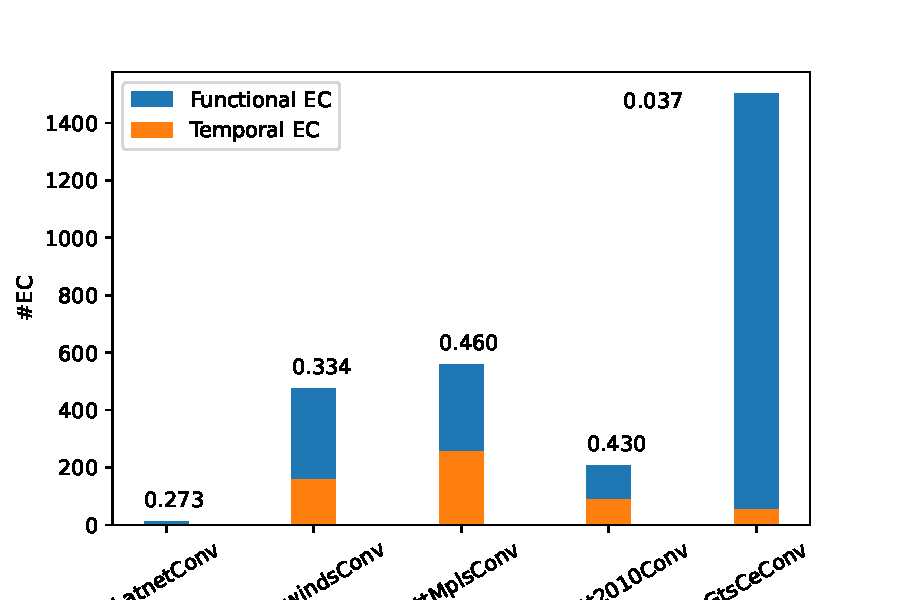
\includegraphics[scale=0.5]{ec}
    \caption{Amount of temporal EC compared to functional EC, label represents ratio}
    \label{fig:ec}
\end{figure}

While we cannot directly compare Tempus with other verifiers (due to difference in verification goal), 
we could use the amount of equivalence class as an indirect proxy of the verifier's behavior and performance.
Therefore, we measured the amount of additional equivalence classes introduced by Tempus in order to 
indirectly compare its overhead in addition to its functional counterparts.
This result is only influenced by the consolidation strategy, since the memoization strategy operates on 
a smaller granularity than equivalence classes.

Our results in Fig. \ref{fig:ec} shows the ratio between the amount of temporal equivalence classes that is 
being re-explored and the amount of functional equivalence class.
We note that we only need to \textbf{re-explore 4\% to 46\% equivalence classes} as an additional overhead 
compared to functional verification.

We conclude that \textbf{consolidation is effective in reducing the amount of equivalence classes that 
needs to be re-explored} in our verification framework.

\subsection{Optimization Analysis}

\begin{table}[h]
    \begin{tabular}{| c | c | c | c | c |}
        \hline
        Top. & \# path & \# path (cons) & \# path (base) & \# conv \\
        \hline
        % Latnet & 0\% & 4.2 \\
        % Highwinds & 97.7\% & 581.41  \\
        % AT\&T & 98.4\% & x \\
        % Uninett & 82.5\% & 108.87 \\
        % GtsCe & 98.2\% & 571.14 \\
        ft4 & 20 & 92 & 251 & 204 \\
        ft6 & 81 & 1,278 & 7,857 & 855 \\
        ft8 & 304 & 42,892 & 500,195 & 3280 \\
        ft10 & 25 & 456,700 & 6,669,169 & 175 \\
        ft12 & 36 & 14,367,491 & 288,537,289 & 252 \\
        ft14* & 49 & 23,767,482 & 323,686,008 & 343 \\
        ft16* & 64 & 21,272,060 & 261,254,848 & 448 \\
        ft24* & 144 & 19,064,581 & 132,197,345 & 1008 \\
        ft32* & 256 & 15,926,575 & 75,783,276 & 1792 \\
        \hline
    \end{tabular}
    \caption{Effectiveness metric}
    \label{tab:analysis}
\end{table}

Up to this point, we have demonstrated that consolidation and memoization are two effective strategies in 
reducing the verification duration and amount of convolution procedure that needs to be done.
However, the results also show that their effectiveness varies depending on the topology.

\subsubsection{Why is Fat Tree 10 better than Fat Tree 4?}
To analyze what affects the effectiveness of our optimization technique, we will start by explaining 
one peculiar result in our evaluation: despite having a bigger size, the temporal verification runtime 
of fat tree with $k = 10$ is faster than $k = 4$.

This is due to the fact that the shortest path in $k = 10$ is a lot more diverse than that of $k = 4$.
In a 3-tier Fat Tree topology, an edge node could reach another pod's edge node in at least 4 hops.
The amount of this shortest path is $(k/2)^2$, which is the same as the number of core node.

We could see from Table \ref{tab:analysis} that when $k \geq 10$, the amount of unique path explored by the 
functional verifier is exactly the same as the number of core node. 
Combined with the fact that the average amount of convolution per path is 7 (which suggests that the path 
length is 4), means that the functional verifier only produces equivalence classes that consisted of only 
different combination of these shortest paths.

When $k < 10$ however, the functional verifier also needs to produce equivalence classes that results 
in a longer convergent paths in order to reach the same accuracy level.
in Fat Tree, this is usually marked by a visit to another aggregation node in another pod. 
We could see from Table \ref{tab:analysis} that when $k < 10$, the amount of of convolution per path is more 
than 7 (which suggests that a path longer than 4 hops exist).

\subsubsection{Generalization}
From the insight of this particular result, we could draw two properties in a general network that could 
determine the runtime of our verifier.

The first one is the \textbf{amount of possible paths}.
If the amount of possible paths between a src-dst pair in a given topology is small, then the functional 
verification step would produce fewer equivalence classes and end early.
While most of our evaluated topology had a lot of possible paths, one exception to this is LatNet, which 
only have 3 possible paths.

The second is whether the src-dst pair in a given topology would \textbf{produce paths that are "symmetric"}.
By symmetric, we mean that the routing and load balancing method produce a lot of identical equivalence class 
and / or equivalence class that share the same path.
As our explanation about Fat Tree 10 suggests, larger Fat Tree has a lot of path with the same length.
This would result in a lot of symmetrical equivalence classes under ECMP.
Our optimization techniques could identify this symmetry and reduce the amount of convolution in the temporal 
verification step.

%TODO: path enumeration?

\section{Limitation and Future Works} \label{sec:fut}
\textbf{Addressing Distribution Independence}
The convolution of two probability distributions assumes that the two distributions are \textit{independent}
of each other.
While we accept this as a limitation of our model, latency in real networks (particularly the latency of two 
queues in the network) might be dependent of each other.

Queuing theory has laid some ground work to describe the asymptotic behavior of such queuing network.
However, they assume some information about the incoming traffic and can only describe a network with a 
particular traffic or delay distribution, like poisson.

Thus, eliminating the independence assumption without demanding an unwieldy amount of information from 
the user while maintaining (or even improving) the accuracy of the model remains an open challenge and an 
interesting future direction.

\textbf{Optimizing Functional Verification}
In our verifier, we built our temporal verifier on top of an existing functional verifier design.
While it makes the design of the verifier simpler, since there is clear separation of concern, there 
might be some performance benefit to gain if we integrate these two parts further.

While we have proposed and evaluated optimization techniques for the temporal verification step, 
integrating this optimization to the functional verification step -- perhaps by consolidating the 
equivalence classes before it is brought to the temporal verification stage in some way -- might make 
our approach more scalable.

While our evaluation shows that the functional verification stage is not the bottleneck of our design, 
discovering the symmetry in the exploration state that might accomplish this task might bring an interesting 
insight to the network verification community in general.

\section{Related Works} \label{sec:rel}
\textbf{Deterministic Data and Control Plane Verifier}
There has been a substantial body of work concerning the functional behavior of routers
with a given Forwarding Information Base (FIB) or Routing Information Base (RIB).

Prior works like HSA \cite{hsa}, NetKAT \cite{netkat}, and VeriFlow \cite{veriflow} focuses on verifying the 
current data plane forwarding behavior against some property.
While useful in some real-time cases, these tools are not built to explore the many
possible forwarding table given an enumeration of failure cases.

Control plane verifiers such as ARC \cite{arc}, Minesweeper \cite{minesweeper}, and 
Tiramisu \cite{tiramisu} focuses on verifying the various data plane states that 
could be produced by a control plane configuration over multiple failure scenarios.
Many researchers has built on top of this idea, such as DNA \cite{dna} where they 
focuses on verifying the change in property in the event of configuration update.

As comprehensive as it is, both approaches only considers the functional behavior 
of the network (e.g. reachability, loop detection) and they traditionally verify 
the stated properties in a black or white fashion, only determining whether a given 
property is violated or not.

As a result, unlike Tempus, its usefulness does not extend into the use cases of 
verifying SLA, where such binary guarantees are often rightfully avoided in favor 
of a probabilistic and/or quantitative agreement.

\textbf{Probabilistic Verifier}
More recent works have tried to address this very issue.
Works like ProbNetKAT \cite{probnetkat} (a probabilistic verifier based on NetKAT 
\cite{netkat}), NetDice \cite{netdice}, and SRE \cite{sre} provides 
the user ability to define probabilistic failure model, where a given component 
of the network can fail with a given probability.

However, most of them still considers the functional property of the network as the 
main focus. 
While they are useful in verifying certain types of SLA (e.g. availability), they don't 
focus on more quantitative aspect of the network (e.g. bandwidth, latency).

\textbf{Quantitative Verifier}
Some recent works are an exception to this trend, however.
Works like QARC \cite{qarc} (a quantitative verifier based on 
ARC \cite{arc}) has developed a framework to verify one particular quantitative 
property: excess bandwidth on a certain link.
While QARC is a deterministic verifier, like Tempus, they focuses on a more quantitative 
property. 
Unlike Tempus however, this work is orthogonal to verifying latency and thus complementary 
to Tempus.

%TODO: ICNA paper?

\textbf{Network Calculus}
One promising concept with regards to performance metric verification is the theoretical 
framework of network calculus.
Network calculus aims to provide a framework to analyze the bandwidth and latency guarantee 
of a flow.
It could model link capacities, background traffic, and congestion control.
CCAC \cite{ccac}, for example, has developed a tool based on this framework to help explain 
the various behavior of a congestion control system.

While providing a strong theoretical background in latency verification, this framework 
primarily deals with guaranteeing bounds deterministically.
It also requires the user to provide more information compared to \tool, since the user 
need to provide the cummulative arrival and departure curve over time.



\section{Conclusion} \label{sec:conc}
\begin{itemize}
    \item Tempus is a scalable latency SLA verifier. It could probabilistically verify in the order of minutes
    \item Consolidation and memoization is an effective optimization strategy, although the exact magnitude of 
        its effectiveness will depend on the network topology, specifically on the amount of paths and their 
        length.
\end{itemize}

\bibliography{cit}
\bibliographystyle{ieeetr}
\end{document}